\documentclass[11pt,preprint]{elsarticle}

\usepackage{lmodern}
%%%% My spacing
\usepackage{setspace}
\setstretch{1.2}
\DeclareMathSizes{12}{14}{10}{10}

% Wrap around which gives all figures included the [H] command, or places it "here". This can be tedious to code in Rmarkdown.
\usepackage{float}
\let\origfigure\figure
\let\endorigfigure\endfigure
\renewenvironment{figure}[1][2] {
    \expandafter\origfigure\expandafter[H]
} {
    \endorigfigure
}

\let\origtable\table
\let\endorigtable\endtable
\renewenvironment{table}[1][2] {
    \expandafter\origtable\expandafter[H]
} {
    \endorigtable
}


\usepackage{ifxetex,ifluatex}
\usepackage{fixltx2e} % provides \textsubscript
\ifnum 0\ifxetex 1\fi\ifluatex 1\fi=0 % if pdftex
  \usepackage[T1]{fontenc}
  \usepackage[utf8]{inputenc}
\else % if luatex or xelatex
  \ifxetex
    \usepackage{mathspec}
    \usepackage{xltxtra,xunicode}
  \else
    \usepackage{fontspec}
  \fi
  \defaultfontfeatures{Mapping=tex-text,Scale=MatchLowercase}
  \newcommand{\euro}{€}
\fi

\usepackage{amssymb, amsmath, amsthm, amsfonts}

\def\bibsection{\section*{References}} %%% Make "References" appear before bibliography


\usepackage[numbers]{natbib}

\usepackage{longtable}
\usepackage[margin=2.3cm,bottom=2cm,top=2.5cm, includefoot]{geometry}
\usepackage{fancyhdr}
\usepackage[bottom, hang, flushmargin]{footmisc}
\usepackage{graphicx}
\numberwithin{equation}{section}
\numberwithin{figure}{section}
\numberwithin{table}{section}
\setlength{\parindent}{0cm}
\setlength{\parskip}{1.3ex plus 0.5ex minus 0.3ex}
\usepackage{textcomp}
\renewcommand{\headrulewidth}{0.2pt}
\renewcommand{\footrulewidth}{0.3pt}

\usepackage{array}
\newcolumntype{x}[1]{>{\centering\arraybackslash\hspace{0pt}}p{#1}}

%%%%  Remove the "preprint submitted to" part. Don't worry about this either, it just looks better without it:
\makeatletter
\def\ps@pprintTitle{%
  \let\@oddhead\@empty
  \let\@evenhead\@empty
  \let\@oddfoot\@empty
  \let\@evenfoot\@oddfoot
}
\makeatother

 \def\tightlist{} % This allows for subbullets!

\usepackage{hyperref}
\hypersetup{breaklinks=true,
            bookmarks=true,
            colorlinks=true,
            citecolor=blue,
            urlcolor=blue,
            linkcolor=blue,
            pdfborder={0 0 0}}


% The following packages allow huxtable to work:
\usepackage{siunitx}
\usepackage{multirow}
\usepackage{hhline}
\usepackage{calc}
\usepackage{tabularx}
\usepackage{booktabs}
\usepackage{caption}


\newenvironment{columns}[1][]{}{}

\newenvironment{column}[1]{\begin{minipage}{#1}\ignorespaces}{%
\end{minipage}
\ifhmode\unskip\fi
\aftergroup\useignorespacesandallpars}

\def\useignorespacesandallpars#1\ignorespaces\fi{%
#1\fi\ignorespacesandallpars}

\makeatletter
\def\ignorespacesandallpars{%
  \@ifnextchar\par
    {\expandafter\ignorespacesandallpars\@gobble}%
    {}%
}
\makeatother


% definitions for citeproc citations
\NewDocumentCommand\citeproctext{}{}
\NewDocumentCommand\citeproc{mm}{%
\href{\#cite.\detokenize{#1}}{#2}\nocite{#1}}

\makeatletter
% allow citations to break across lines
\let\@cite@ofmt\@firstofone
% avoid brackets around text for \cite:
\def\@biblabel#1{}
\def\@cite#1#2{{#1\if@tempswa , #2\fi}}
\makeatother
\newlength{\cslhangindent}
\setlength{\cslhangindent}{1.5em}
\newlength{\csllabelwidth}
\setlength{\csllabelwidth}{3em}
\newenvironment{CSLReferences}[2] % #1 hanging-indent, #2 entry-spacing
{\begin{list}{}{%
	\setlength{\itemindent}{0pt}
	\setlength{\leftmargin}{0pt}
	\setlength{\parsep}{0pt}
	% turn on hanging indent if param 1 is 1
	\ifodd #1
	\setlength{\leftmargin}{\cslhangindent}
	\setlength{\itemindent}{-1\cslhangindent}
	\fi
	% set entry spacing
	\setlength{\itemsep}{#2\baselineskip}}}
{\end{list}}

\usepackage{calc}
\newcommand{\CSLBlock}[1]{\hfill\break\parbox[t]{\linewidth}{\strut\ignorespaces#1\strut}}
\newcommand{\CSLLeftMargin}[1]{\parbox[t]{\csllabelwidth}{\strut#1\strut}}
\newcommand{\CSLRightInline}[1]{\parbox[t]{\linewidth - \csllabelwidth}{\strut#1\strut}}
\newcommand{\CSLIndent}[1]{\hspace{\cslhangindent}#1}


\urlstyle{same}  % don't use monospace font for urls
\setlength{\parindent}{0pt}
\setlength{\parskip}{6pt plus 2pt minus 1pt}
\setlength{\emergencystretch}{3em}  % prevent overfull lines
\setcounter{secnumdepth}{5}

%%% Use protect on footnotes to avoid problems with footnotes in titles
\let\rmarkdownfootnote\footnote%
\def\footnote{\protect\rmarkdownfootnote}
\IfFileExists{upquote.sty}{\usepackage{upquote}}{}

%%% Include extra packages specified by user

%%% Hard setting column skips for reports - this ensures greater consistency and control over the length settings in the document.
%% page layout
%% paragraphs
\setlength{\baselineskip}{12pt plus 0pt minus 0pt}
\setlength{\parskip}{12pt plus 0pt minus 0pt}
\setlength{\parindent}{0pt plus 0pt minus 0pt}
%% floats
\setlength{\floatsep}{12pt plus 0 pt minus 0pt}
\setlength{\textfloatsep}{20pt plus 0pt minus 0pt}
\setlength{\intextsep}{14pt plus 0pt minus 0pt}
\setlength{\dbltextfloatsep}{20pt plus 0pt minus 0pt}
\setlength{\dblfloatsep}{14pt plus 0pt minus 0pt}
%% maths
\setlength{\abovedisplayskip}{12pt plus 0pt minus 0pt}
\setlength{\belowdisplayskip}{12pt plus 0pt minus 0pt}
%% lists
\setlength{\topsep}{10pt plus 0pt minus 0pt}
\setlength{\partopsep}{3pt plus 0pt minus 0pt}
\setlength{\itemsep}{5pt plus 0pt minus 0pt}
\setlength{\labelsep}{8mm plus 0mm minus 0mm}
\setlength{\parsep}{\the\parskip}
\setlength{\listparindent}{\the\parindent}
%% verbatim
\setlength{\fboxsep}{5pt plus 0pt minus 0pt}



\begin{document}



\begin{frontmatter}  %

\title{Predictors of loan defaults}

% Set to FALSE if wanting to remove title (for submission)




\author[Add1]{24693197}
\ead{}





\address[Add1]{Stellenbosch University, South Africa}

\cortext[cor]{Corresponding author: 24693197}

\begin{abstract}
\small{
Abstract to be written here. The abstract should not be too long and
should provide the reader with a good understanding what you are writing
about. Academic papers are not like novels where you keep the reader in
suspense. To be effective in getting others to read your paper, be as
open and concise about your findings here as possible. Ideally, upon
reading your abstract, the reader should feel he / she must read your
paper in entirety.
}
\end{abstract}

\vspace{1cm}


\begin{keyword}
\footnotesize{
Multivariate GARCH \sep Kalman Filter \sep Copula \\
\vspace{0.3cm}
}
\footnotesize{
\textit{JEL classification} L250 \sep L100
}
\end{keyword}



\vspace{0.5cm}

\end{frontmatter}

\setcounter{footnote}{0}



%________________________
% Header and Footers
%%%%%%%%%%%%%%%%%%%%%%%%%%%%%%%%%
\pagestyle{fancy}
\chead{}
\rhead{}
\lfoot{}
\rfoot{\footnotesize Page \thepage}
\lhead{}
%\rfoot{\footnotesize Page \thepage } % "e.g. Page 2"
\cfoot{}

%\setlength\headheight{30pt}
%%%%%%%%%%%%%%%%%%%%%%%%%%%%%%%%%
%________________________

\headsep 35pt % So that header does not go over title




\section{\texorpdfstring{Introduction
\label{Introduction}}{Introduction }}\label{introduction}

This report looks at loan default trends using Lending Club data
covering one million anonymised peer-to-peer loans. It looks at the
beliefs the Director wishes to challenge. Namely, that home owners and
people that's been employed more than 10 years have a far lower
probability of default with short term loans, that US States differ
significantly when it comes to a culture of defaulting on short term
loans and that Credit Grades (A - F) provide a great indicator for
whether younger individuals will default or not. Also that interest
rates are also clearly determined by age, occupation and credit scores.

\section*{Data}\label{data}
\addcontentsline{toc}{section}{Data}

\section{Step 1: Data Cleaning and
Exploration}\label{step-1-data-cleaning-and-exploration}

Before any analysis, the data was reduced to the columns relevant to
this analysis and several cleaning steps were applied.

\begin{itemize}
\item
  Two binary outcome variables were created from loan\_status.
  Default\_Flag takes the value 1 for loans charged off or defaulted, 0
  for fully paid, and NA for current loans. These are excluded from
  default rate calculations as their outcome is not yet known.
\item
  Employment length and loan term were stored as text (``6 years'', ``36
  months'') and converted to numeric for analysis.
\item
  Credit grade was set as an ordered factor from A (lowest risk) to G
  (highest risk).
\item
  Credit history length is used a s a proxy for age since there is no
  direct age variable in the dataset. It is derived from
  earliest\_cr\_line and it is used as a proxy since a longer history is
  likely linked to an older borrower.
\item
  Continuous variables with clear outliers were Winsorized at the 1st
  and 99th percentiles. DTI had impossible values ranging from -1 to
  999, and annual income reached as high as \$9.9 million so both
  required capping to prevent extreme values from distorting the
  results.
\end{itemize}

\subsection{Key Risk Drivers}\label{key-risk-drivers}

\subsubsection{Default Rate by Credit
Grade}\label{default-rate-by-credit-grade}

\pandocbounded{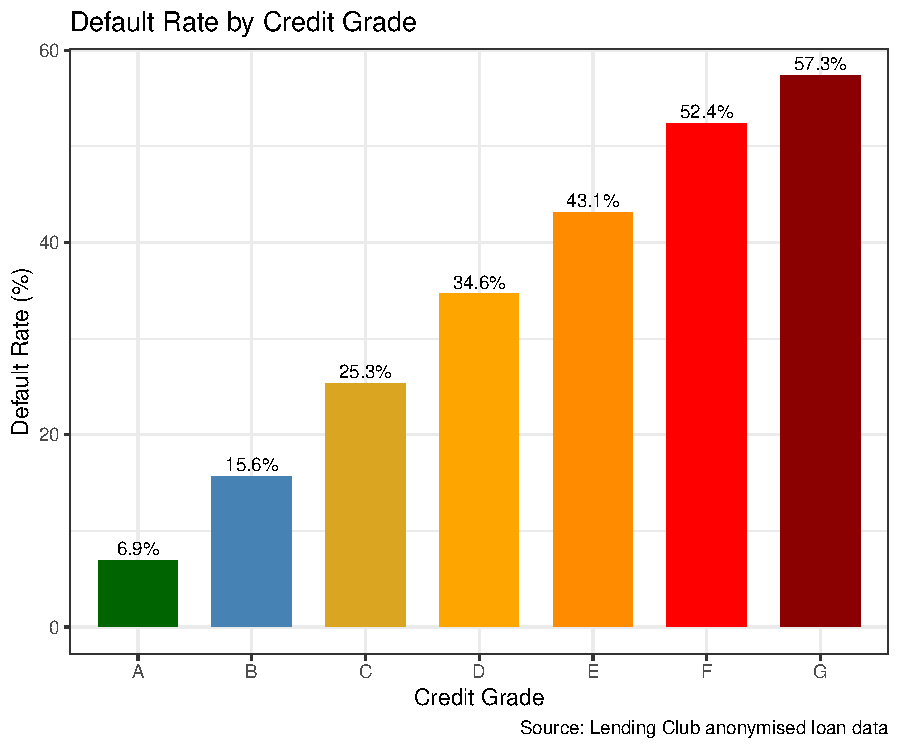
\includegraphics[keepaspectratio,alt={Default rates rise monotonically from Grade A to G, confirming the grading system captures genuine credit risk.}]{Question3_files/Question3_files/figure-latex/plot-grade-1.pdf}}
The plot shows a clear strong relationship between credit grade and
default rate (as expected).

\subsubsection{Default Rate by Loan
Purpose}\label{default-rate-by-loan-purpose}

\begin{figure}
\centering
\pandocbounded{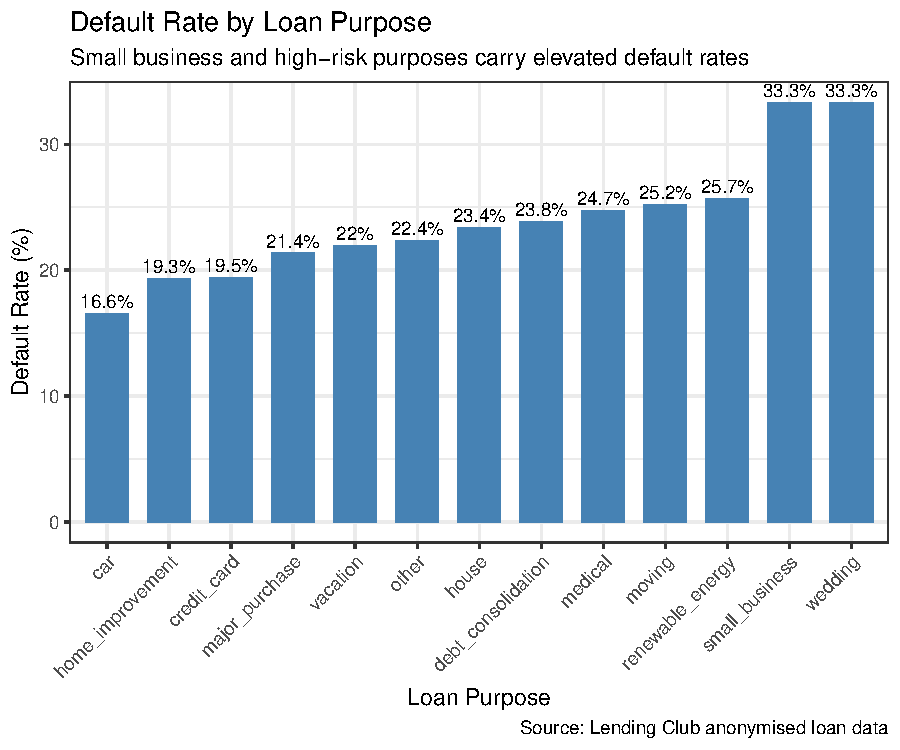
\includegraphics[keepaspectratio,alt={Loan purpose varies substantially in associated default risk.}]{Question3_files/Question3_files/figure-latex/plot-purpose-1.pdf}}
\caption{Loan purpose varies substantially in associated default risk.}
\end{figure}

Car and home improvement loans carry the lowest default rates at around,
while small business and wedding loans sit at the top at. Thus, lenders
should apply greater scrutiny to higher-risk purpose categories when
assessing borrower credibility. This plot provides evidence that loan
purpose is a a good credit risk signal.

\subsection{Evaluating the beliefs}\label{evaluating-the-beliefs}

\subsubsection{Belief: Homeowners and Long-Tenured Employees Default
Less}\label{belief-homeowners-and-long-tenured-employees-default-less}

\begin{figure}
\centering
\pandocbounded{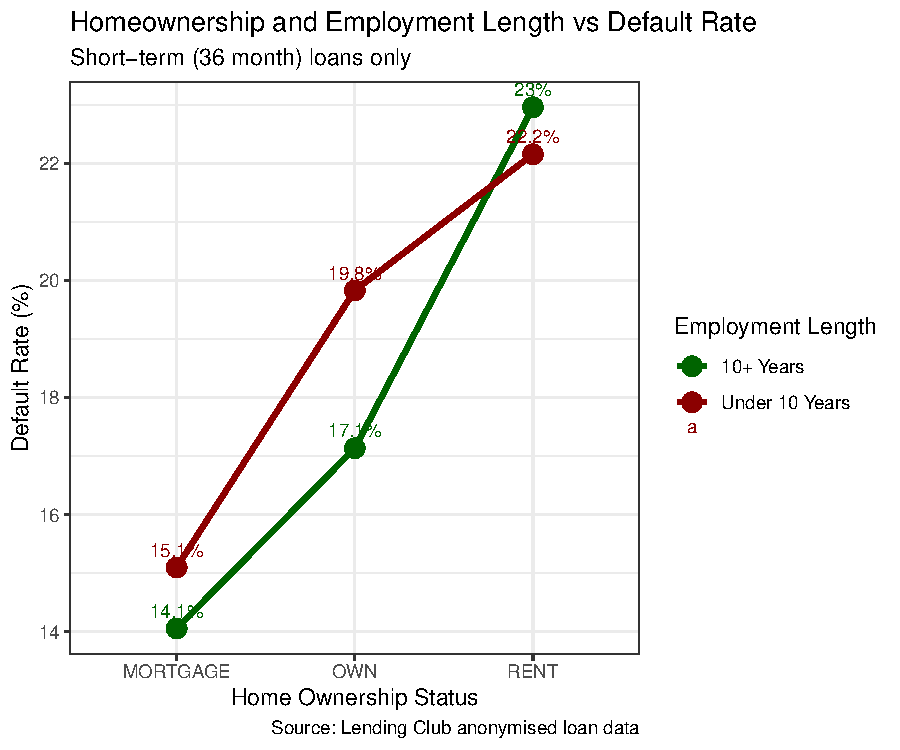
\includegraphics[keepaspectratio,alt={The director's heuristic receives only partial support.}]{Question3_files/Question3_files/figure-latex/plot-heuristic-1.pdf}}
\caption{The director's heuristic receives only partial support.}
\end{figure}

The above plot somewhat confirms this belief since borrowers employed
for 10 or more years show slightly lower default rates (lower by \(1%
\)). This difference is really small so this belief is only partly
supported by the data. On the other hand, homeowners (those with over
and under 10 years of employment) have higher default rates than
borrowers.

\subsubsection{Belief: US States Differ Significantly in Default
Culture}\label{belief-us-states-differ-significantly-in-default-culture}

\begin{figure}
\centering
\pandocbounded{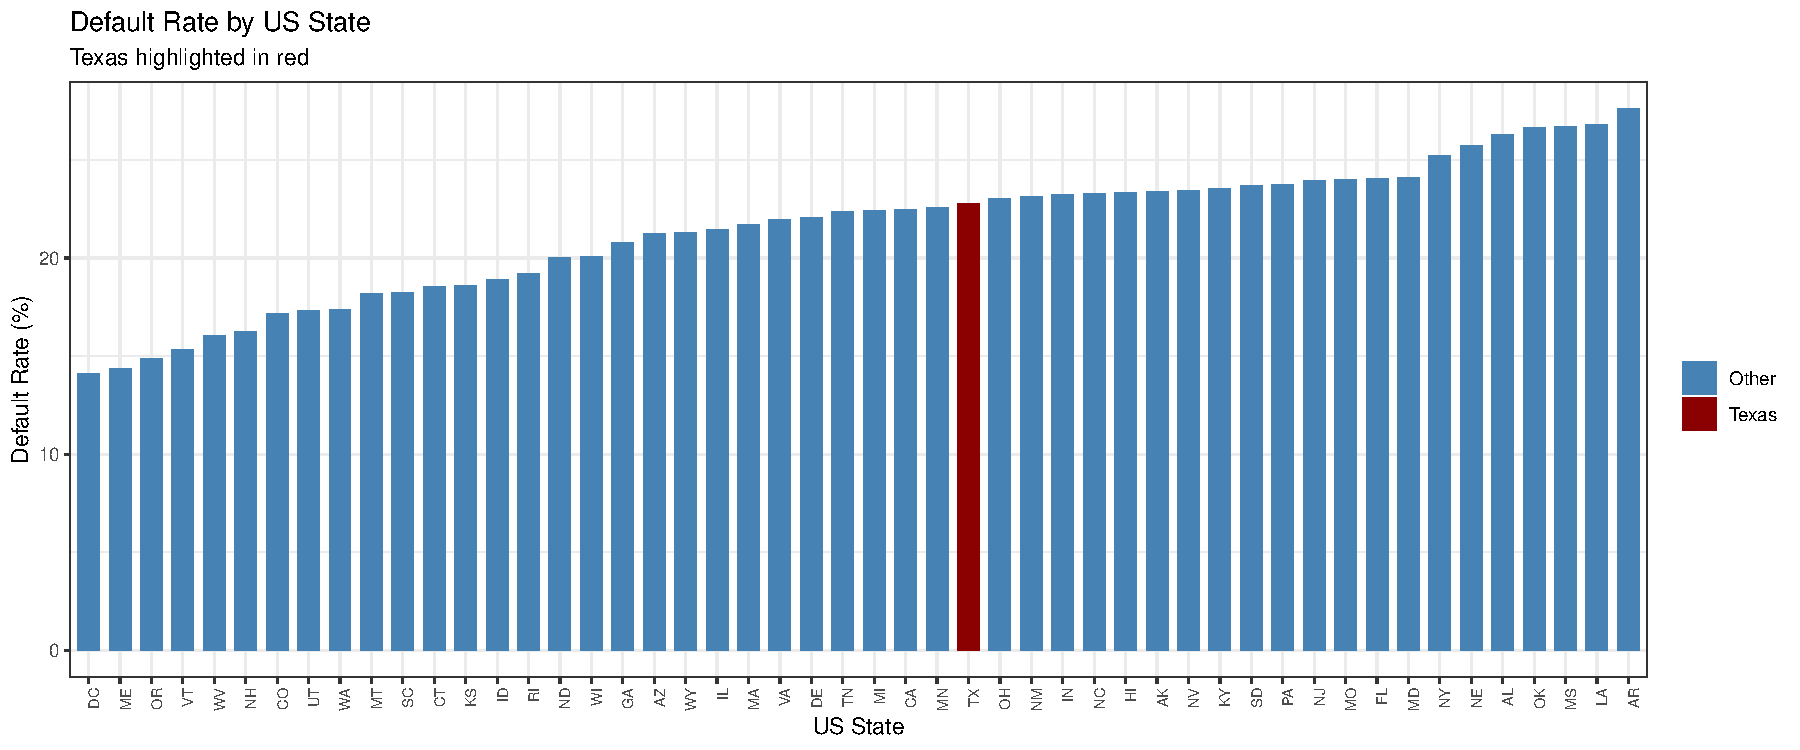
\includegraphics[keepaspectratio,alt={Default rates vary across states but Texas sits close to the national average.}]{Question3_files/Question3_files/figure-latex/plot-state-1.pdf}}
\caption{Default rates vary across states but Texas sits close to the
national average.}
\end{figure}

This belief is more closely supported by the data because default rates
range from around \(14%
\) to about \(27%/28%
\). This means that US states do in fact differ significantly in default
culture. Texas (labeled TX on the x-axis) sits slightly above the the
average when looking at the bigger picture.

\subsubsection{Belief: Credit Grades (A - F) Predict Whether Younger
Individuals Will Default
Well}\label{belief-credit-grades-a---f-predict-whether-younger-individuals-will-default-well}

\pandocbounded{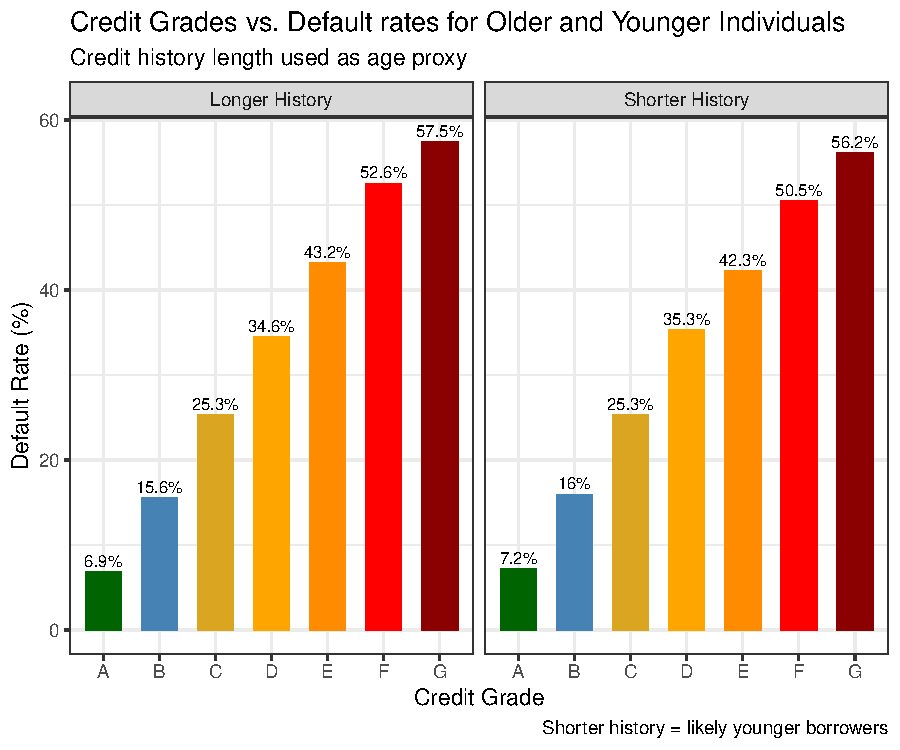
\includegraphics[keepaspectratio]{Question3_files/Question3_files/figure-latex/plot-grade-age-1.pdf}}

The credit grading system has the same relationship as before for both
younger (shorter credit history) and older (longer credit history)
individuals. This relationship is that default rates increase with lower
credit grades. The differences between older and younger individuals
default rates' is very small. For higher grades, younger individuals
have a slightly higher default rating while for higher grades it is the
opposite. Thus, there is no evidence from the data to support the belief
that grades work better or worse for younger borrowers specifically.

\subsubsection{Belief: Interest Rates Are Determined by Age, Occupation,
and Credit
Scores}\label{belief-interest-rates-are-determined-by-age-occupation-and-credit-scores}

\pandocbounded{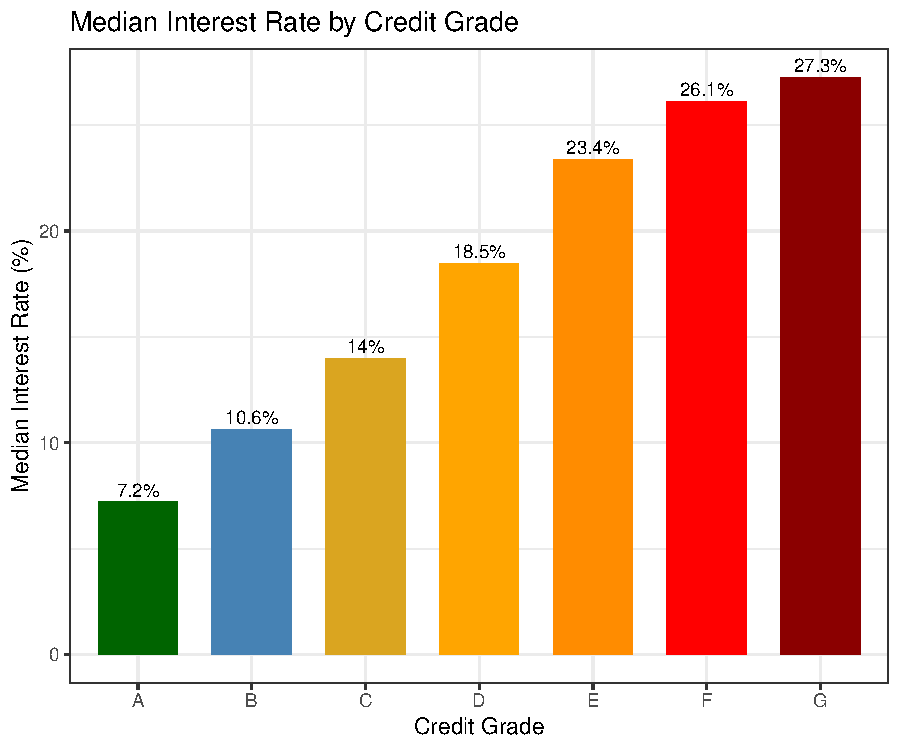
\includegraphics[keepaspectratio]{Question3_files/Question3_files/figure-latex/plot-int-rate-1.pdf}}

From this graph it is obvious that credit rating is an obvious
determinant of interest rates. From the basic understanding of interest
rates and credit ratings, this correlation makes sense, because a lower
credit rating means there is a higher risk of default. Thus, the risk is
compensated for by a higher interest rate (compared to higher credit
ratings).

\section{Conclusion}\label{conclusion}

This report analysed one million Lending Club loans to assess default
risk drivers and evaluate four beliefs held by the Credit Institute in
Texas.

Credit grade is the strongest predictor of default, with a clear and
consistent relationship between grade and default rate. Loan purpose
also carries meaningful risk signal car and home improvement loans have
the lowest default rates while small business and wedding loans sit at
the top.

The evidence on the four beliefs of the Institute is relatively mixed.
The homeownership and length of employment belief is only partially
supported because borrowers with 10 or more years of employment default
slightly less, but the difference is small. The belief that US states
differ in default culture is supported, with default rates ranging from
around 14\% to 27\% across states and Texas sits close to the national
average. Credit grades predict default consistently for both younger and
older borrowers with very small differences between the two groups.
There is no evidence that grades work better or worse for younger
individuals specifically. Finally, credit grade is clearly the dominant
driver of interest rates, but the independent roles of age and
occupation cannot be assessed as neither variable is directly available
in the dataset.

\newpage

\section*{References}\label{references}
\addcontentsline{toc}{section}{References}

\protect\phantomsection\label{refs}

\section*{Appendix}\label{appendix}
\addcontentsline{toc}{section}{Appendix}

\subsection*{Appendix A}\label{appendix-a}
\addcontentsline{toc}{subsection}{Appendix A}

Some appendix information here

\subsection*{Appendix B}\label{appendix-b}
\addcontentsline{toc}{subsection}{Appendix B}

\bibliography{Tex/ref}





\end{document}
